\documentclass{article}
\usepackage[utf8]{inputenc}
\usepackage{amsmath}
\usepackage{amssymb}
\usepackage{graphicx}
\usepackage{xcolor}
\newcommand\xk{x^{\left(n\right)}}
\newcommand\xkn{x^{\left(n+1\right)}}
\newcommand\xz{x^{\left(0\right)}}

\begin{document}
\section*{Newton's method for $F\left(x\right) := \arctan\left(x\right) = 0$}
\subsection*{8-3.a}
We are tasked with finding the smallest positive initial guess $\xz$ for which Newton's method does not converge when it is applied to $F\left(x\right) = \arctan\left(x\right)$. Let us first write down the Newton iteration in this case. We have
\begin{equation*}
    F'\left(x\right) = \frac{1}{1 + x^{2}}
\end{equation*}
the Newton iteration is given as
\begin{align*}
    \xkn = \xk - \frac{F\left(\xk\right)}{F'\left(\xk\right)} = \xk - \frac{\arctan\left(\xk\right)}{\frac{1}{1 + \left(\xk\right)^{2}}} &= \xk - \arctan\left(\xk\right)\left(1+ \left(\xk\right)^{2}\right) \\
    &= \xk \underbrace{- \arctan\left(\xk\right) + \left(\xk\right)^{2}\arctan\left(\xk\right)}_{\text{determines convergence / divergence}}
\end{align*}
We can see that that the underlined term is what determines the behaviour of the Newton iteration, because we have
\begin{equation*}
    \arctan\left(\xz\right) \leq \left(\xz\right)^{2}\arctan\left(\xz\right) \implies \xz \leq x^{\left(1\right)} \implies x^{\left(1\right)} \leq x^{\left(2\right)} \implies \dots \implies \xk \leq \xkn
\end{equation*}
hence divergent behaviour. Let us look at these two functions to understand when this happens.
\begin{figure}[!hbt]
    \centering
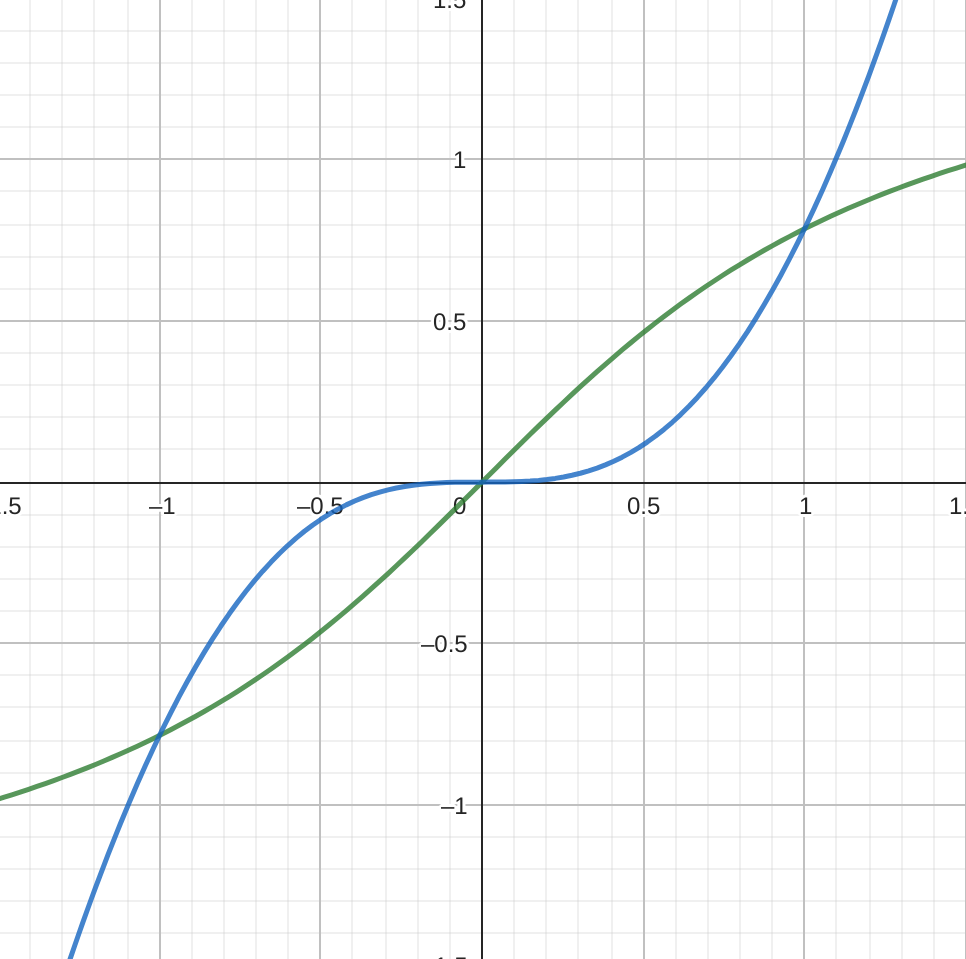
\includegraphics[width=0.5\linewidth]{arctan_vs_x2arctan.png}
\end{figure}
\begin{align*}
    \color{green} f\left(x\right) &\color{green}= \arctan\left(x\right) \\
    \color{blue}g\left(x\right) &\color{blue}= x^{2}\arctan\left(x\right)
\end{align*}
We can see that the initial guess threshold is located around $\left\lvert \xz \right\rvert < 1$. Let us find this value mathematically. For this purpose we are interested in finding the zero of the function
\begin{equation*}
    h\left(x\right)= \arctan\left(x\right) - x^{2}\arctan\left(x\right)
\end{equation*}
this function looks as follows an describes the intersects of the above functions.
\begin{figure}[!hbt]
    \centering
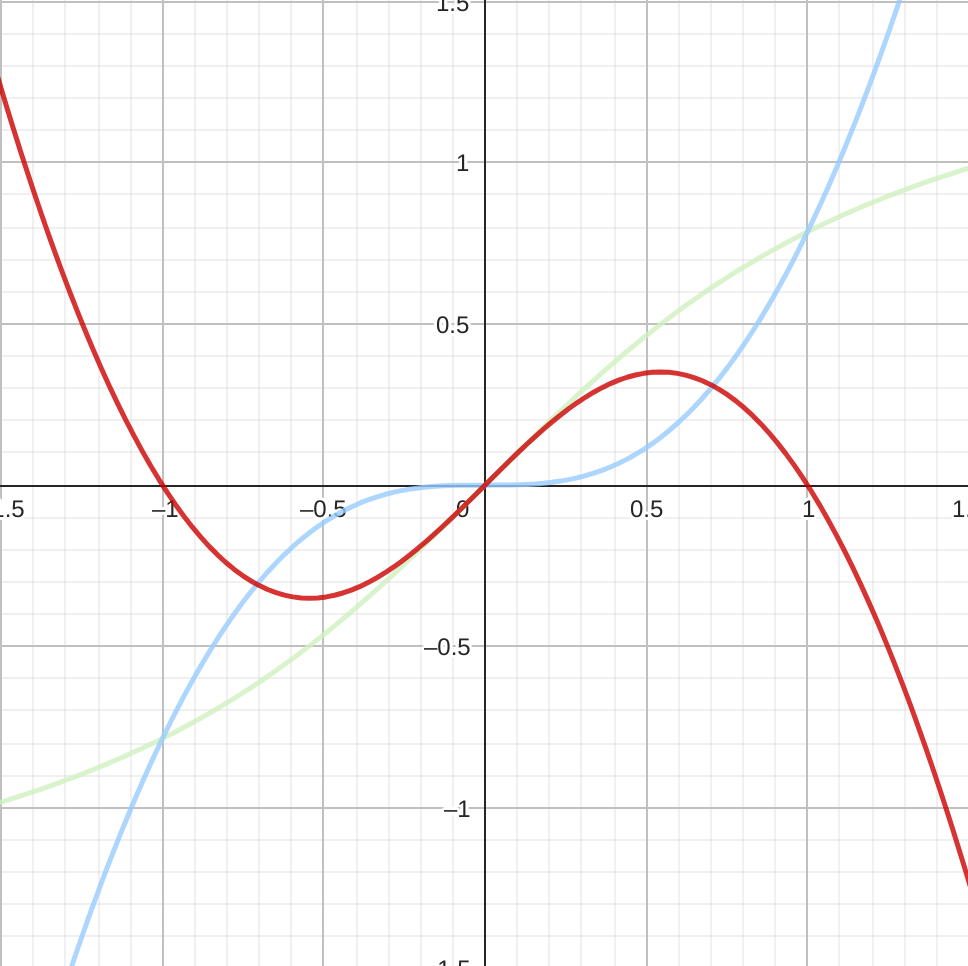
\includegraphics[width=0.5\linewidth]{8-3function2.png}
\end{figure}
\begin{equation*}
    \color{red}h\left(x\right)= \arctan\left(x\right) - x^{2}\arctan\left(x\right)
\end{equation*}
We can see that for $x=0$ we have 
\begin{align*}
    &f\left(0\right) = \arctan\left(0\right) = 0 \\
    &g\left(0\right) = 0^{2}\cdot \arctan\left(0\right) = 0
\end{align*}
and for $x=1$ we have
\begin{align*}
    &f\left(1\right) = \arctan\left(1\right) \\
    &g\left(1\right) = 1^{2} \cdot \arctan\left(1\right) = \arctan\left(1\right) = f\left(1\right) 
\end{align*}
Hence we can say that the Newton iteration for $\arctan\left(x\right)$ only converges if the initial guess is in the interval $\left(-1,1\right)$. In other words
\begin{equation*}
    \text{Newton iteration converges for } \arctan\left(x\right) =  0 \Longleftrightarrow \xz\in \left(-1,1\right)
\end{equation*}

\pagebreak

\subsection*{8-3.b} 
We are now tasked with finding such an approximation of $\xz$ again using the Newton's method. We implement for this purpose the function \verb|newton_arctan| with initial guess per default \verb|x0_ = 2.0|. We will iterate until we are close enough to zero that any new update is smaller than the numerical limit. For this purpose we will use $\\[2mm]$
\verb|std::numeric_limits<double>::epsilon()|
$\\[1mm]$
We then compute in each step the next iteration according to the Newton iteration for the function $h$ found above given by
\begin{equation*}
    h\left(x\right) = \arctan\left(x\right) - x^{2}\arctan\left(x\right)
\end{equation*}
We choose the initial guess of $\xz = 2.0$, because otherwise we will find $0.0$ as result, which is a bit pointless, as that is the fixpoint itself. The derivative of $h$ is given by (we apply the product rule and the summation rule for derivation)
\begin{align*}
    h'\left(x\right) &= \frac{1}{1+x^{2}} - 2x\cdot \arctan\left(x\right) - x^{2} \frac{1}{1+x^{2}} \\
    &= \frac{1}{1+x^{2}} -2x\cdot \arctan\left(x\right) - \frac{x^{2}}{1+x^{2}} \\
    &= \frac{1-x^{2}}{1+x^{2}}-2x\cdot \arctan\left(x\right) \\
    &= \frac{1-x^{2} -2x\cdot\arctan\left(x\right) -2x^{3}\cdot arctan\left(x\right)}{1+x^{2}} \\
    &= -\frac{-1+x^{2}+2\left(x+x^{3}\right)\cdot \arctan\left(x\right)}{1+x^{2}}
\end{align*}
This approach differs a bit from the one made int the solution, as they use that the smallest possible initial guess $\xz$ for which the Newton's method does not converge it the one where we have $x^{\left(1\right)} = -\xz$ and we oscillate back and forth between these values. This then leads to the equation
\begin{equation*}
    x^{\left(1\right)} = x^{\left(0\right)} - \frac{f\left(\xz\right)}{f'\left(\xz\right)} = \xz - \left(1 + \left(\xz\right)^{2}\right)\arctan\left(\xz\right) = -\xz
\end{equation*}
from which we can deduce that $\xz$ must be a zero of the function
\begin{equation*}
    \tilde{h}\left(x\right) = 2x - \left(1+x^{2}\right)\cdot \arctan\left(x\right) 
\end{equation*}
with
\begin{equation*}
\tilde{h}'\left(x\right) = 1 - 2x\cdot \arctan\left(x\right)
\end{equation*}
this is much easier to compute, but also one must first derive this, we will hence supply implementations for both ways.

\pagebreak

\noindent The following implementation does converge and produces a result after a long time but it converges only slowly which will most of the time result in code expert ending the process.

\begin{figure}[!hbt]
    \centering
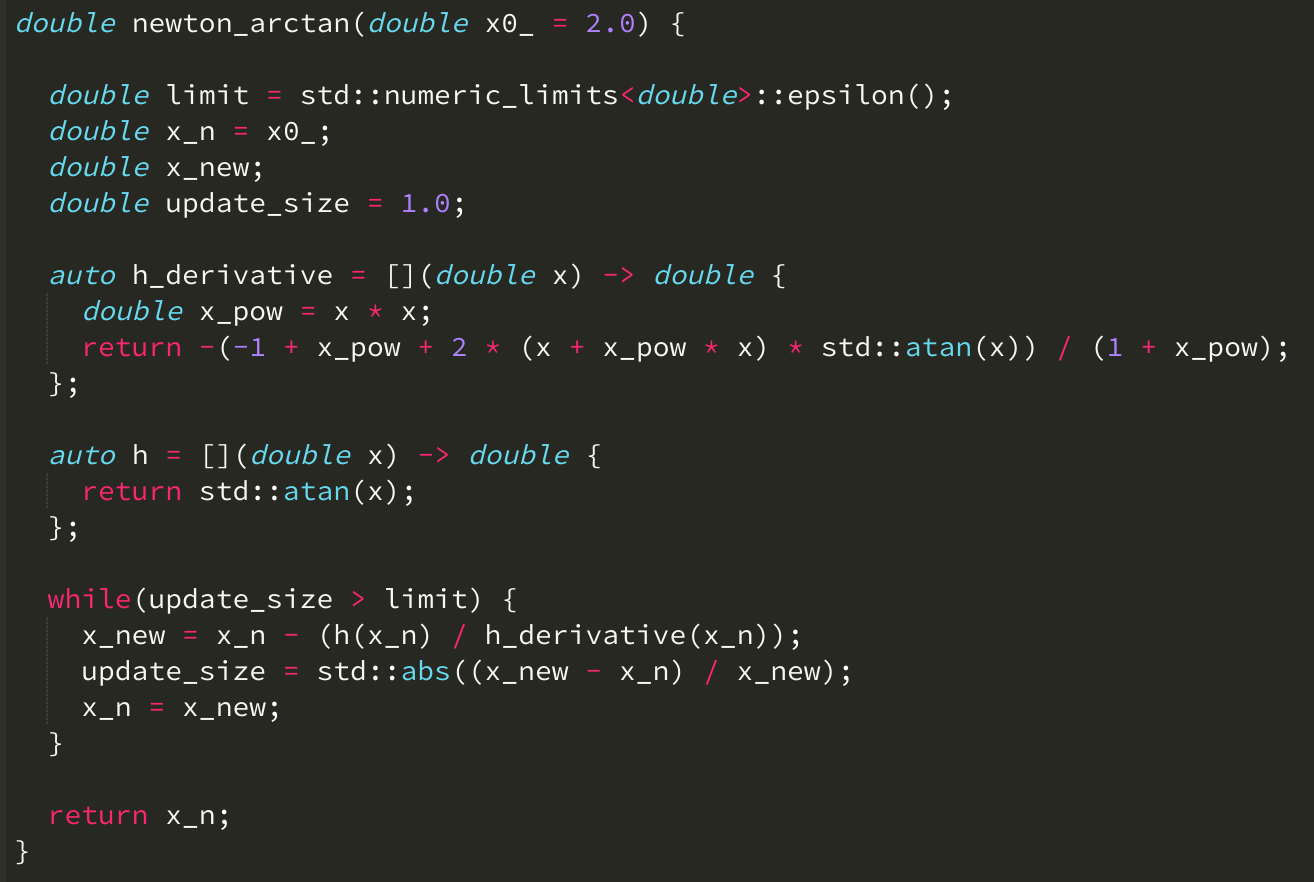
\includegraphics[width=1.0\linewidth]{8-3.b.png}
\end{figure}

\noindent A code that produces results and is fast is given below and it uses the (better) solution discussed above.

\begin{figure}[!hbt]
    \centering
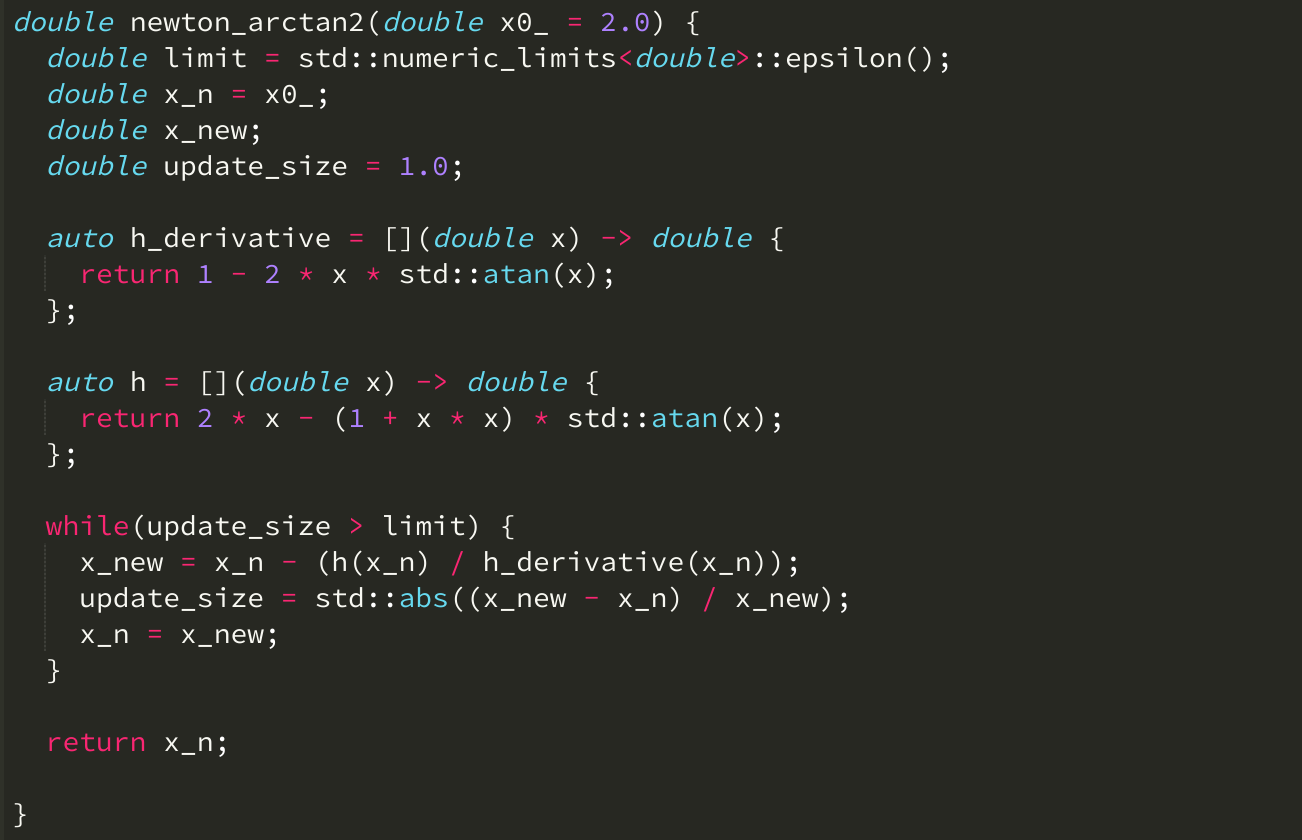
\includegraphics[width=1.0\linewidth]{8-3.b2.png}
\end{figure}

\end{document}
